\documentclass[parskip=full,11pt,twoside]{scrartcl}
\usepackage[utf8]{inputenc}

\title{Simulator für wiederholte Spiele}
\author{Sebastian Feurer, Peter Koepernik, Luc Mercatoris,\\Christian Schorr, Pierre Toussing}

% section numbers in margins:
\renewcommand\sectionlinesformat[4]{\makebox[0pt][r]{#3}#4}

% header & footer
\usepackage{scrlayer-scrpage}
\lofoot{\today}
\refoot{\today}
\pagestyle{scrheadings}

\usepackage[sfdefault,light]{roboto}
\usepackage[T1]{fontenc}
\usepackage[german]{babel}
\usepackage[yyyymmdd]{datetime} % must be after babel
\renewcommand{\dateseparator}{-} % ISO8601 date format
\usepackage{hyperref}
\usepackage{amsmath} % for $\text{}$
\usepackage{amssymb}
\usepackage[nameinlink]{cleveref}
\crefname{figure}{Abb}{Abb}
\usepackage[section]{placeins}
\usepackage{xcolor}
\usepackage{graphicx}
\hypersetup{
	pdftitle={Pflichtenheft},
	bookmarks=true,
}
\usepackage{csquotes}

\newcommand\urlpart[2]{$\underbrace{\text{\texttt{#1}}}_{\text{#2}}$}

\usepackage{pflichtenheft}

\def\adapt{Adaptionsschritt}
\def\adapts{Adaptionsschritte}

\def\segment{Segment}
\def\segments{Segmente}

\begin{document}
\maketitle

\section{Einleitung}

Ziel dieses Projekts ist die Entwicklung einer Simulationsumgebung für wiederholte Spiele. Sie ist aus der Forschung motiviert und für den Einsatz in der Forschung ausgelegt. Die Simulationsumgebung wird verwendet, um das Entstehen von Gleichgewichtszuständen bei wiederholten Spielen mehrerer Agenten zu untersuchen. 

Es folgt eine Erläuterung des dem Simulator zugrundeliegenden Ablaufs. Dazu sei auch auf \cref{} verwiesen.

Eine Simulation besteht aus mehreren Wiederholungen. Eine Wiederholung beginnt mit der Initialisierung der Agenten mit Strategien, Kapital und Gruppenzugehörigkeit. Anzahl der Agenten, Zuweisungsverfahren von Anfangsstrategien und Anfangskapital sowie Gruppeneinteilung werden vom Nutzer spezifiziert. Insbesondere legt der Nutzer die Menge aller möglichen Strategien fest. Danach folgen wiederholt \adapts, bis sich ein Gleichgewicht eingestellt hat oder eine konfigurierbare Höchstzahl an \adapts n erreicht ist. Ein \adapt\ besteht aus einer festen Zahl an Runden. In jeder Runde werden zunächst gemäß eines konfigurierbaren Algorithmus' Paare aus Agenten gebildet. Diese spielen dann gemäß ihrer aktuellen Strategie das dieser Simulation zugrundeliegende Stufenspiel. Nach Ablauf der Runden wird der Erfolg jedes Agenten in den zurückliegenden Runden quantifiziert und daraus eine Rangliste aller Agenten erstellt. Die Agenten passen nun ihre Strategien gemäß eines vom Nutzer spezifizierbaren Adaptionsmechanismus an. Ziel ist dabei nicht die Maximierung des Absolutkapitals, sondern eine möglichst hohe Position auf der Rangliste.

Nachdem alle Wiederholungen abgeschlossen sind, erfolgt die Ausgabe der Ergebnisse der einzelnen Wiederholungen. Wenn sich ein Gleichgewicht eingestellt hat, werden die Zahl der durchgeführten \adapts, die endgültigen Strategien und die endgültige Rangliste ausgegeben.

\pagebreak
\section{Kriterien}
% Diese Section sollte kurz und knapp "für Manager" sein
% und auf eine Seite passen.

\subsection{Muss}

\criterium{Starten einer Simulation}{crt:startsim}	

Der Nutzer kann eine Simulation starten, welche dann mit den aktuell festgelegten Parametern durchgeführt wird.

\criterium{Ausgabe der Simulationsergebnisse}{crt:simresults_std}

Nach Durchführung einer Simulation wird für jede der Wiederholungen ausgegeben, ob sich ein Gleichgewicht eingestellt hat. Falls ja, werden die Zahl der durchgeführten \adapts, die endgültigen Strategien und die endgültige Rangliste ausgegeben.

\criterium{Abbrechen einer Simulation}{crt:interruptsim}

Der Nutzer kann eine laufende Simulation abbrechen.

\criterium{Anpassen von Simulationsparametern}{crt:simparam_std}

Der Nutzer hat die Möglichkeit, die folgenden Simulationsparameter festzulegen:
\begin{itemize} \itemsep -10pt
\item Anzahl der Agenten
\item zugrundeliegendes Stufenspiel
\item Anzahl verschiedener Gruppen und jeweils Anzahl zugehöriger Agenten
\item Zuweisungsverfahren für initiale Strategien
\item Menge aller möglichen Strategien
\item Zuweisungsverfahren für initiales Kapital
\item Algorithmus zur Bildung von Paaren beim Beginn einer Runde
\item Erfolgsquantifizierung zur Erstellung der Rangliste am Ende eines \adapt s
\item Adaptionsmechanismus, nach dem Agenten am Ende eines \adapt s ihre Strategien anpassen
\end{itemize}

\subsection{Kann}

\criteriumOptional{Detailliertere Ausgabe}{crt:simresults_add}
Nach Ablauf einer Simulation können für jede Wiederholung Rangliste und Strategien am Ende aller Adaptionsschritte eingesehen werden.

\criteriumOptional{Anpassen der Abbruchbedingungen}{crt:exitcondition}
Es können mehrere Kriterien für den Abbruch einer Wiederholung verwendet werden.

\criteriumOptional{Erweiterte Gruppenfunktionalität}{crt:groupfunc}
Gruppen und die Menge der gruppenlosen Agenten können jeweils in \segments\ unterteilt werden. Für jedes \segment\ können Zuweisungsverfahren für initiale Strategien und initiales Kapital separat festgelegt werden.

\criteriumOptional{Speichern und Laden von Konfigurationen}{crt:saveloadconfig}
Eine Konfiguration kann als Datei abgespeichert werden. Eine solche Konfigurationsdatei kann wiederum geladen werden.

\criteriumOptional{Erstellen eigener Strategien}{crt:createstrat}
Es können eigene Strategien erstellt werden.

\criteriumOptional{Erstellen eigener Stufenspiele}{crt:creategame}
Es können eigene Stufenspiele erstellt werden.

\subsection{Abgrenzung}

\criteriumNot{Kein alternativer Simulationsablauf}{crt:not_altsim}
Der zugrundeliegende Ablauf der Simulation, wie in der Einleitung erklärt, kann nicht verändert werden.

\criteriumNot{Keine komplexen Stufenspiele}{crt:not_complexgames}
Als Stufenspiele sind nur solche zugelassen, die sich als \(2 \times 2\) - Bimatrix mit konstanten Auszahlungen darstellen lassen.

\pagebreak

%%%%%%%%%%%
\section{Funktionale Anforderungen}

\functionality{Festlegen der Menge aller möglichen Strategien}{fnc:stratset}
\fulfills{crt:simparam_std}
Der Nutzer kann bei der Konfiguration einer Simulation die Menge aller Strategien festlegen, die in dieser Simulation von Agenten verwendet werden können.

Dazu befindet sich im Konfigurationsfenster ein 'Strategie hinzufügen'-Knopf. Darunter befindet sich eine Liste aller bereits hinzugefügten Strategien (siehe \cref{}). Bei Betätigen des 'Strategie hinzufügen'-Knopfes öffnet sich ein Fenster mit einer Liste aller im System hinterlegten Strategien. Mittels üblicher \textsf{CTRL}- und \textsf{SHIFT}-Klick-Funktionalität können eine oder mehrere Strategien ausgewählt werden. Bereits hinzugefügte Strategien sind ausgegraut und können nicht ausgewählt werden (siehe \cref{}). Beim Betätigen des 'Bestätigen'-Knopfes wird das Fenster geschlossen und alle ausgewählten Strategien werden zu der Liste hinzugefügt. Beim Betätigen des 'Abbrechen'-Knopfes wird das Fenster geschlossen und keine Strategien werden hinzugefügt. Unter der Liste der hinzugefügten Strategien befindet sich eine Checkbox mit der Bezeichnung 'gemischte Strategien'. Ist diese aktiviert, so können Agenten im Laufe der Simulation gemischte Strategien entwickeln. Ist die Checkbox deaktiviert, werden nur reine Strategien verwendet.

In der Liste der ausgewählten Strategien befindet sich neben jeder Strategie ein '\(\circleddash\)'-Knopf. Wird dieser betätigt, wird die Strategie aus der Liste entfernt.

Wird der Mauszeiger im Auswahlfenster oder in der Liste über eine Strategie bewegt, so öffnet sich ein Tooltip mit einer kurzen Beschreibung der Strategie.

Abgesehen von selbst erstellten Strategien sind folgende Strategien im System hinterlegt:
\begin{itemize} \itemsep -10pt
\item Tit-for-tat
\item Grim
\item Kooperation mit Agenten mit ähnlichem Absolutkapital\footnote{Das Absolutkapital zweier Agenten ist ähnlich, genau dann wenn sich der Rang der Agenten, aufgelistet nach Absolutkapital, höchstens um \(20\%\) der Gesamtzahl aller Agenten unterscheidet.}, ansonsten keine Kooperation
\item Tit-for-tat mit Agenten mit ähnlichem Absolutkapital, ansonsten keine Kooperation
\item Keine Kooperation mit Agenten mit höherem Absolutkapital, ansonsten tit-for-tat
\item Keine Kooperation mit Agenten mit niedrigerem Absolutkapital, ansonsten tit-for-tat
\item Kooperation mit Agenten derselben Gruppenzugehörigkeit, ansonsten keine Kooperation
\item Tit-for-tat mit Agenten derselben Gruppenzugehörigkeit, ansonsten keine Kooperation
\item Immer Kooperation
\item Nie Kooperation
\end{itemize}

\functionality{Konfiguration von Anzahl und Größe der Gruppen}{fnc:groups}
\fulfills{crt:simparam_std}
Der Nutzer hat die Möglichkeit, die Anzahl verschiedener Gruppen in einem Simulationsdurchlauf festzulegen. Weiterhin kann er angeben, wie viele Agenten den einzelnen Gruppen und wie viele Agenten keiner Gruppe zugehörig sind.

Dazu muss im Konfigurationsfenster der Abschnitt 'Gruppeneinstellungen' durch Drücken des Knopfes am linken Rand des entsprechend benannten Separators ausgeklappt werden (siehe \cref[{}). Voreingestellt sind null Gruppen. Eine neue Gruppe kann durch Betätigen des 'Gruppe hinzufügen'-Knopfes hinzugefügt werden (siehe \cref{}). Jeder Gruppe wird bei Erstellung eine zufällige, unter allen Gruppen eindeutige Farbe zugeordnet. Ist die maximale Anzahl von fünf Gruppen erreicht, ist der 'Gruppe hinzufügen'-Knopf ausgegraut und kann nicht mehr betätigt werden.

Eine Gruppe wird beim Hinzufügen mit null Mitgliedern initialisiert. Die Anzahl der Mitglieder einer Gruppe kann über den Multislider links des 'Gruppe hinzufügen'-Knopfes verändert werden. Für jede Gruppe befindet sich ein entsprechend gefärbter Schiebe-Knopf auf dem Multislider. Der Slider-Abschnitt links des Knopfes wird ebenfalls mit der Gruppenfarbe gefärbt. Die relative Größe jeder Gruppe entspricht genau der relativen Größe des entsprechend gefärbten Abschnitts auf dem Slider. Der rechtsgelegenste Abschnitt ist weiß gefärbt und gibt die Anzahl der gruppenlosen Agenten an. Über jedem Abschnitt wird die Zahl von Agenten angezeigt, die diesem Abschnitt angehören (siehe \cref{}). Wird durch Verschieben eines Sliders die Größe einer Gruppe verändert, so ändern sich die Größen anderer Gruppen nicht. Beim Vergrößern einer Gruppe sinkt also die Zahl der gruppenlosen Agenten, beim Verkleinern einer Gruppe vergrößert sie sich. Folglich kann keine Gruppe vergrößert werden, wenn bereits alle Agenten einer Gruppe angehören.

Die Abschnitte des Sliders fungieren als Tab-Control. Unterhalb des Sliders befindet sich ein Abschnitt zur Konfiguration der aktuell per Tab-Control ausgewählten Gruppe bzw. der gruppenlosen Agenten (siehe \cref{}). Im Konfigurationsabschnitt einer Gruppe befindet sich ein 'Gruppe löschen'-Knopf. Wird dieser betätigt, öffnet sich ein Bestätigungs-Dialog (siehe \cref{}). Wird in diesem auf 'Abbrechen' gedrückt, schließt sich der Dialog und die Konfiguration bleibt unverändert. Wird auf 'Bestätigen' gedrückt, schließt sich der Dialog und die Gruppe wird gelöscht. Das Tab-Control wechselt zu den gruppenlosen Agenten und die Mitglieder der gelöschten Gruppe werden gruppenlos.

\functionality{Einteilung von Gruppen in \segments}{fnc:segments}
\fulfills{crt:groupfunc}
Der Nutzer kann jede Gruppe und die Menge der gruppenlosen Agenten in ein bis fünf \segments\ unterteilen. Für jedes \segment\ können die Zuweisungsverfahren für initiale Strategien und initiales Kapital separat konfiguriert werden.

Die Unterteilung erfolgt im Konfigurationsabschnitt einer Gruppe bzw. der gruppenlosen Agenten. Am oberen Ende des Abschnittes befindet sich eine Überschrift '\segment einstellungen', darunter ein Multislider und ein '\segment\ hinzufügen'-Knopf (siehe \cref{}). Voreingestellt ist ein Segment. Ein neues Segment kann durch Betätigen des '\segment\ hinzufügen'-Knopfes hinzugefügt werden. Ist die maximale Anzahl von fünf \segments n erreicht, ist der '\segment\ hinzufügen'-Knopf ausgegraut und kann nicht mehr betätigt werden. Für jedes hinzugefügte Segment erscheint auf dem Multislider ein Schiebe-Knopf. Wie bei den Gruppeneinstellungen entspricht jeder Abschnitt auf dem Slider einem \segment. Durch Verschieben der Schiebe-Knöpfe kann so die Größe der \segments\ verändert werden. Die Abschnitte fungieren als Tab-Control, und unter dem Slider befindet sich ein Konfigurationsabschnitt für das aktuell ausgewählte \segment. Der Konfigurationsabschnitt enthält die Einstellungen für das Zuweisungsverfahren für initiale Strategien und initiales Kapital.

Am unteren Ende des Konfigurationsabschnittes eines \segment s befindet sich ein '\segment\ löschen'-Knopf. Betätigen des Knopfes öffnet einen Bestätigungs-Dialog. Wird in diesem auf 'Abbrechen' gedrückt, so schließt sich der Dialog und die Konfiguration bleibt unverändert. Wird in dem Dialog auf 'Bestätigen' gedrückt, so schließt sich der Dialog und das \segment\ wird entfernt. Gibt es nur noch ein \segment, so ist der '\segment\ löschen'-Knopf ausgegraut und kann nicht betätigt werden.

\functionality{Konfiguration des Zuweisungsverfahrens für initiale Strategien}{fnc:initialstrat}
\fulfills{crt:simparam_std}
\fulfills{crt:groupfunc}
Der Nutzer kann das Zuweisungsverfahren für die initialen Strategien der Agenten beim Beginn einer Wiederholung einstellen. Diese Einstellung findet für jedes \segment\ einer Gruppe und für jedes \segment\ der gruppenlosen Agenten separat statt.

Die Einstellung erfolgt in dem Konfigurationsabschnitt eines \segment s. Dort befindet sich ein mit 'Initiale Strategien' beschrifteter Unterabschnitt. In diesem befinden sich zwei nebeneinander angeordnete List-Boxen (siehe \cref{}). Die Linke ist beschriftet mit 'Alle Strategien', die Rechte mit 'Gewählte Strategien'. In der linken Box sind alle Strategien aufgelistet, die der Nutzer für diese Simulation zugelassen hat. Die rechte Box ist zunächst leer. Per üblicher \textsf{CTRL}- und \textsf{SHIFT}-Klick-Funktionalität können eine oder mehrere Strategien in der linken Box ausgewählt werden. Betätigen des 'Hinzufügen'-Knopfes zwischen den beiden Boxen entfernt alle ausgewählten Strategien aus der linken Box und fügt sie in die rechte Box ein. Analog können Strategien in der rechten Box ausgewählt und mittels Betätigen des 'Entfernen'-Knopfes aus der rechten Box entfernt und in die Linke wieder eingefügt werden.

Zu Beginn jeder Wiederholung im so konfigurierten Simulationsablauf wird jedem Agent aus dem aktuell konfigurierten \segment\ zufällig eine Strategie aus der Liste der gewählten Strategien zugeordnet. Ist diese Liste leer, werden den Agenten zufällige Strategien aus der Menge aller zugelassenen Strategien zugeordnet. Insbesondere werden Agenten immer mit reinen Strategien initialisiert.

\functionality{Konfiguration des Zuweisungsverfahrens für initiales Kapital}{fnc:initialcap}
\fulfills{crt:simparam_std}
\fulfills{crt:groupfunc}
Der Nutzer kann das Zuweisungsverfahren für das initiale Kapital der Agenten beim Beginn einer Wiederholung einstellen. Diese Einstellung findet für jedes \segment\ einer Gruppe und für jedes \segment\ der gruppenlosen Agenten separat statt.

Die Einstellung erfolgt in dem Konfigurationsabschnitt eines \segment s. Dort befindet sich ein mit 'Initiales Kapital' beschrifteter Unterabschnitt (siehe \cref{}). Mittels Radiobuttons kann eine der folgenden Wahrscheinlichkeitsverteilungen gewählt werden:
\begin{itemize}
\item Gleichverteilung
\item Binomialverteilung
\item Poissonverteilung
\item festes Ergebnis
\end{itemize}
Unter den Radiobuttons befinden sich Eingabemöglichkeiten zur Parametrisierung der aktuell gewählten Verteilung, eine kurze Beschreibung und ein Graph der Verteilung. Voreingestellt ist das feste Ergebnis \(0\), also kein Anfangskapital.

Für die Gleichverteilung müssen die beiden Intervallgrenzen \(a,b \in \mathbb{N}_0, \ a < b\) in Textfeldern angegeben werden. Voreingestellt ist \(a = 0, b = 100\) (siehe \cref{}).

Bei der Binomialverteilung müssen die Intervallgrenzen \(a,b \in \mathbb{N}_0, \ a < b\) in Textfeldern und der Parameter \(p \in (0,1)\) mittels Slider angegeben werden. Voreingestellt ist \(a = 0, b = 100, p = 0.5\) (siehe \cref{}).

Bei der Poisson-Verteilung muss der Parameter \(\lambda \in \mathbb{N}_0\) in einem Textfeld angegeben werden. Voreingestellt ist \(\lambda = 50\) (siehe \cref{}).

Beim festen Ergebnis muss der Parameter \(a \in \mathbb{N}_0\), der das feste Ergebnis angibt, in einem Textfeld angegeben werden. Voreingestellt ist \(a = 0\) (siehe \cref{}).

Bei fehlerhafter Eingabe eines Parameters wird die Eingabe auf den nächsten zugelassene Wert abgeändert.

Zu Beginn jeder Wiederholung im so konfigurierten Simulationsablauf wird jedem Agent aus dem aktuell konfigurierten \segment\ ein zufälliger Betrag als initiales Kapital zugewiesen, gezogen aus der eingestellten Wahrscheinlichkeitsverteilung.

%%%%%%%%%%%
\section{Nicht-Funktionale Anforderungen}

\nonFunctionality{Modernes Design}{nfc:design}

Das Design soll modern und seriös wirken.

\nonFunctionality{Persistenz}{nfc:persistence}

Sollten in Zukunft Erweiterungen oder Updates notwendig werden,
müssen die Daten (Kurz-URLs, E-Mailaddressen) erhalten bleiben.

\nonFunctionality{Erweiterbarkeit}{nfc:extensibility}

Das Produkt muss dahingehend erweiterbar sein,
das die Liste der E-Mail-URL Abbildung von authentifizierten Nutzern
abgerufen werden kann.
Wie das genau implementiert wird, ist nicht Teil dieses Projekts.

%%%%%%%%%%%
\section{Tests}

\test{Kurz-URL Erstellen}{tst:create}
\tests{fnc:login}

\teststep{Besucher \enquote{Zoe Washburne} hat einen Browser geöffnet.}
{Zoe navigiert auf die Homepage \texttt{http://atu.rl/}.}
{Die Homepage wird angezeigt wie in \cref{fig:homepage}.}

\teststep{Zoe hat einen Facebook-Account.}%
{Zoe drückt den \enquote{Login via Facebook} Knopf.}%
{Zoe wird eingeloggt und auf die Erstellseite wie in \cref{fig:form} weitergeleitet.}

\teststep{}
{Zoe befüllt das Feld \enquote{URL} mit \texttt{sehrlangedomain.com/undganzlangeURL.html} und drückt auf \enquote{Kurz-URL erstellen}.}%
{Ihr wird eine Kurz-URL angezeigt wie z.B.\ \texttt{atu.rl/abc}
 wie in \cref{fig:generated}.
 Statt \enquote{abc}, dürfen beliebige andere Buchstaben und Zahl angezeigt werden, allerdings exakt drei.}

\teststep{}
{Zoe navigiert auf die eben generierte Kurz-URL, z.B.\ \texttt{http://atu.rl/abc}.}
{Sie wird zu \texttt{sehrlangedomain.com/undganzlang  eURL.html} weitergeleitet.}

\test{Betreiberinfos lesen}{tst:tmg}
\tests{fnc:impressum-link}
\tests{fnc:datenschutz-link}

\teststep{Besucher \enquote{Jayne Cobb} ist auf der Homepage}
{Er folgt dem Link mit dem Text \enquote{Datenschutz}}
{Ein Text mit allen Datenschutzinformationen wird ihm angezeigt.}

\teststep{}
{Jayne folgt dem Link mit dem Text \enquote{Impressum}}
{Ein Text mit Informationen des Betreibers wird ihm angezeigt.}

%%%%%%%%%%%%%
\pagebreak
\appendix

\section{Seitenentwürfe}

% made via https://gomockingbird.com/projects/mnf0cwf/4gXVnC

\begin{figure}[hb]
%\fbox{
\includegraphics[width=\textwidth]{image/login.png}}
\caption{\label{fig:homepage}
Homepage mit Login-Funktion
}
\end{figure}

\begin{figure}[hb]
%\fbox{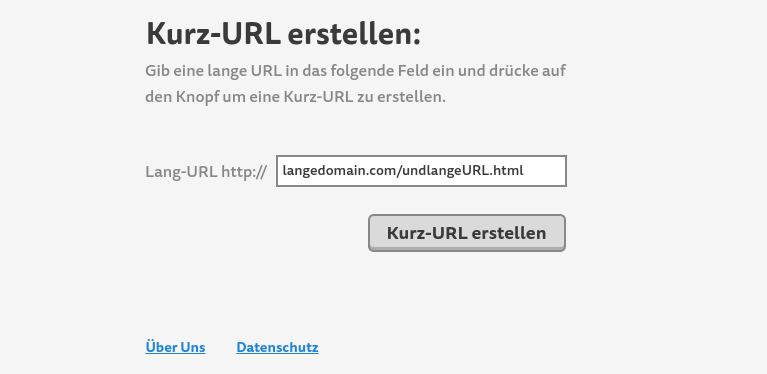
\includegraphics[width=\textwidth]{image/form.png}}
\caption{\label{fig:form}
Formular zur Generierung einer Kurz-URL.
Getestet beispielsweise in \testlink{tst:create}.
}
\end{figure}

\begin{figure}[hb]
%\fbox{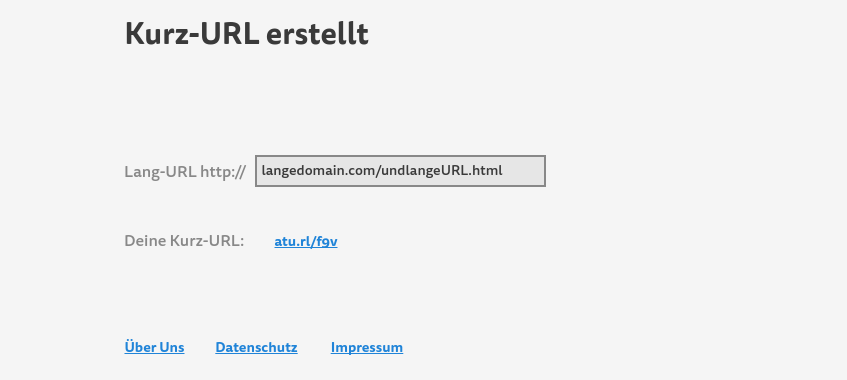
\includegraphics[width=\textwidth]{image/generated.png}}
\caption{\label{fig:generated}
Anzeige der generierten Kurz-URL.
Das Textfeld mit der Lang-URL kann nicht geändert werden.
}
\end{figure}

\section{Glossar}

\textbf{Gleichgewicht}:
Ein Gleichgewicht im Simulationsablauf ist erreicht, wenn keiner der Agenten mehr seine Strategie ändert.

\textbf{Stufenspiel:}
Ein spieltheoretisches Spiel, welches sich als Bimatrix darstellen lässt. (z.B. das Gefangenen-Dilemma)

\textbf{Erfolg:}
Der Erfolg eines Agenten in einer Folge von Runden wird aus dessen Kapitalauszahlungen in diesen Runden berechnet. Er ist Konfigurationsparameter der Simulation. Beispiel ist die Summe aller Auszahlungen.

\textbf{Kapital:}
Jedem Agenten wird im Laufe einer Wiederholung eine Zahl zugeordnet, die sich aus dem Initialisierungswert zu Beginn der Wiederholung und der Summe der Auszahlungen aus den Stufenspielen der bisherigen Runden zusammensetzt.

\textbf{Gruppenzugehörigkeit:}
In einer Simulation sind die Agenten in eine feste, wohldefinierte Anzahl von Gruppen partitioniert. Die Strategien der Agenten können auf Gruppenzugehörigkeiten Bezug nehmen. Dabei haben zwei Agenten genau dann dieselbe Gruppenzugehörigkeit, wenn beide Mitglieder in derselben Gruppe sind. Insbesondere müssen beide Mitglied in einer Gruppe sein.

\textbf{Gruppenloser Agent:}
Ein Agent, der keiner Gruppe angehört.

\textbf{Nutzer:}
Eine Person, welche das Programm nutzt.

\textbf{Multislider:}
Ein Schieberegler mit mehreren möglichen Schiebe-Knöpfen.

\textbf{Slider-Abschnitt:}
Bereich auf dem Slider, der nach rechts und links durch den nächstgelegensten Schiebe-Knopf bzw. den Rand des Sliders begrenzt wird.

\end{document}
